% File SDSS2020_SampleExtendedAbstract.tex
\documentclass[10pt]{article}
\usepackage{sdss2020} % Uses Times Roman font (either newtx or times package)
\usepackage{url}
\usepackage{latexsym}
\usepackage{amsmath, amsthm, amsfonts}
\usepackage{algorithm, algorithmic}
\usepackage{graphicx}
\usepackage{adjustbox}
\graphicspath{{images/}}

\title{Artificial Neural Networks and Deep Learning \\
Homework 1}

\author{
  Nicola Dean \\
  10617541 \\
  {\tt nicola.dean \\
  \tt @mail.polimi.it} \\\And
  Marco Fasanella \\
  10617541 \\
  {\tt marco.fasanella \\
  \tt @mail.polimi.it} \\\And
  Raffaello Fornasiere \\
    10617541 \\
    {\tt raffaello.fornasiere \\
    \tt @mail.polimi.it} \\\And
  Christian Spano \\
  10617541 \\
  {\tt christian.spano \\
  \tt @mail.polimi.it} \\}


\date{}

\begin{document}
\maketitle
%\begin{abstract}

%\end{abstract}

%{\bf Keywords:} VGG16, VGG19, Helpful

\section{Introduction}
--MARCO--

TUTTE LE TECNICHE USATE
come abbiamo pensato di approcciare.
Idee e risultati
Timeline di quello fatto.
Riassiunto delle metodologie e delle CNN
\subsection{Classic Net}


\section{Dataset Helper and Model Helper}
--CHRISTIAN--
Spiegazione delle due classi: \
lista delle funzioni e automatizzazione

\section{First try: vanilla network}
--NICOLA--
-IMG della rete (dal lab) (magari orizzontale)
risultati
considerazioni
\subsection{Batch Normalization}
A first attempt was adding a Batch Normalization + Relu Activation Layer before our Pooling layers.\
This lead to poor result due to the fact that the network was too small.
\subsection{Our homemade CNN}
--- RAFFAELLO---
\subsection{Considerations}
Best result consideration and observations
\section{Transfer Learning and Fine Tuning}
transfer leraning e modelli usati
\subsection{Approach: Freezing Layers}
Idea sulla freezing
\subsection{VGG19}

--MARCO--
Spiegazione modell + prove fatte
\subsubsection{Results}


\begin{table}[ht]
\centering
\begin{adjustbox}{width=240}
\small
\begin{tabular}{|c|l|l|l|l|l}

\hline \bf Freezed Layers & \bf Accuracy & \bf Precision & \bf Recall & \bf F1 \\ \hline
8 & 0.8169 & 0.7989 & 0.7651 & 0.763\\
9 & 0.8225 & 0.8181 & 0.7682 & 0.7776\\
10 & 0.8338 & 0.8161 & 0.7929 & 0.8001\\
11 & 0.7577 & 0.7109 & 0.715 & 0.7048\\
12 & 0.7944 & 0.766 & 0.7504 & 0.7489\\
13 & 0.8028 & 0.7806 & 0.754 & 0.7596\\
\hline
\end{tabular}
\end{adjustbox}
\caption{Results with Transfer Learning and Number of freezed layers for VGG19.}
\end{table}


\begin{figure}[ht]
\begin{center}
\centerline{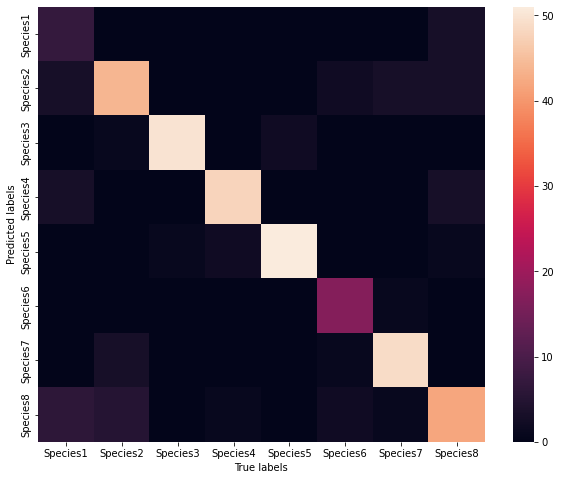
\includegraphics[width=\columnwidth]{VGG19_best}}
\caption{Confusion Matrix of best configuration with VGG19.}
\label{bayespic}
\end{center}
\end{figure}


\subsection{VGG16}
--CHRISTIAN--
Spiegazione modell + prove fatte
\subsubsection{Results}
\subsection{Xception}

\subsection{Other Models}
\subsubsection{Resnet}
--NICOLA--
\subsubsection{GoogleNet}
\subsection{EfficientNet}
--NICOLA--



\section{Ensemble}
--NICOLA--
Approccio
provato a mischiare modelli
          c'era bias perchè avevano seed diversi
\subsubsection{Results}



\section{If we had more time..}
con più tempo cosa avremmo provato




\section{Our Submissions}
\begin{table}[ht]
\centering
\begin{adjustbox}{width=240}
\small
\begin{tabular}{|c|l|l|l|l|l}

\hline \bf Description & \bf Result \\ \hline
a & 0.8169 \\
b & 0.8225 \\

\hline
\end{tabular}
\end{adjustbox}
\caption{Results with Transfer Learning and Number of freezed layers for VGG19.}
\end{table}
%{\bf Footnotes}: Note di sotto.}.
\section{Conclusions}
Considerazioni finali e best model fattoo
\bibliographystyle{sdss2020} % Please do not change the bibliography style
\bibliography{SampleReferencesForExtendedAbstract}

\end{document}
